On previous sections every fragment of the system was described. Figure \ref{fig:System_Architecture} give a look to the common architecture of the system. The basic structure is composed of:
% System architecture image
\begin{figure}[hp]
	\centering
	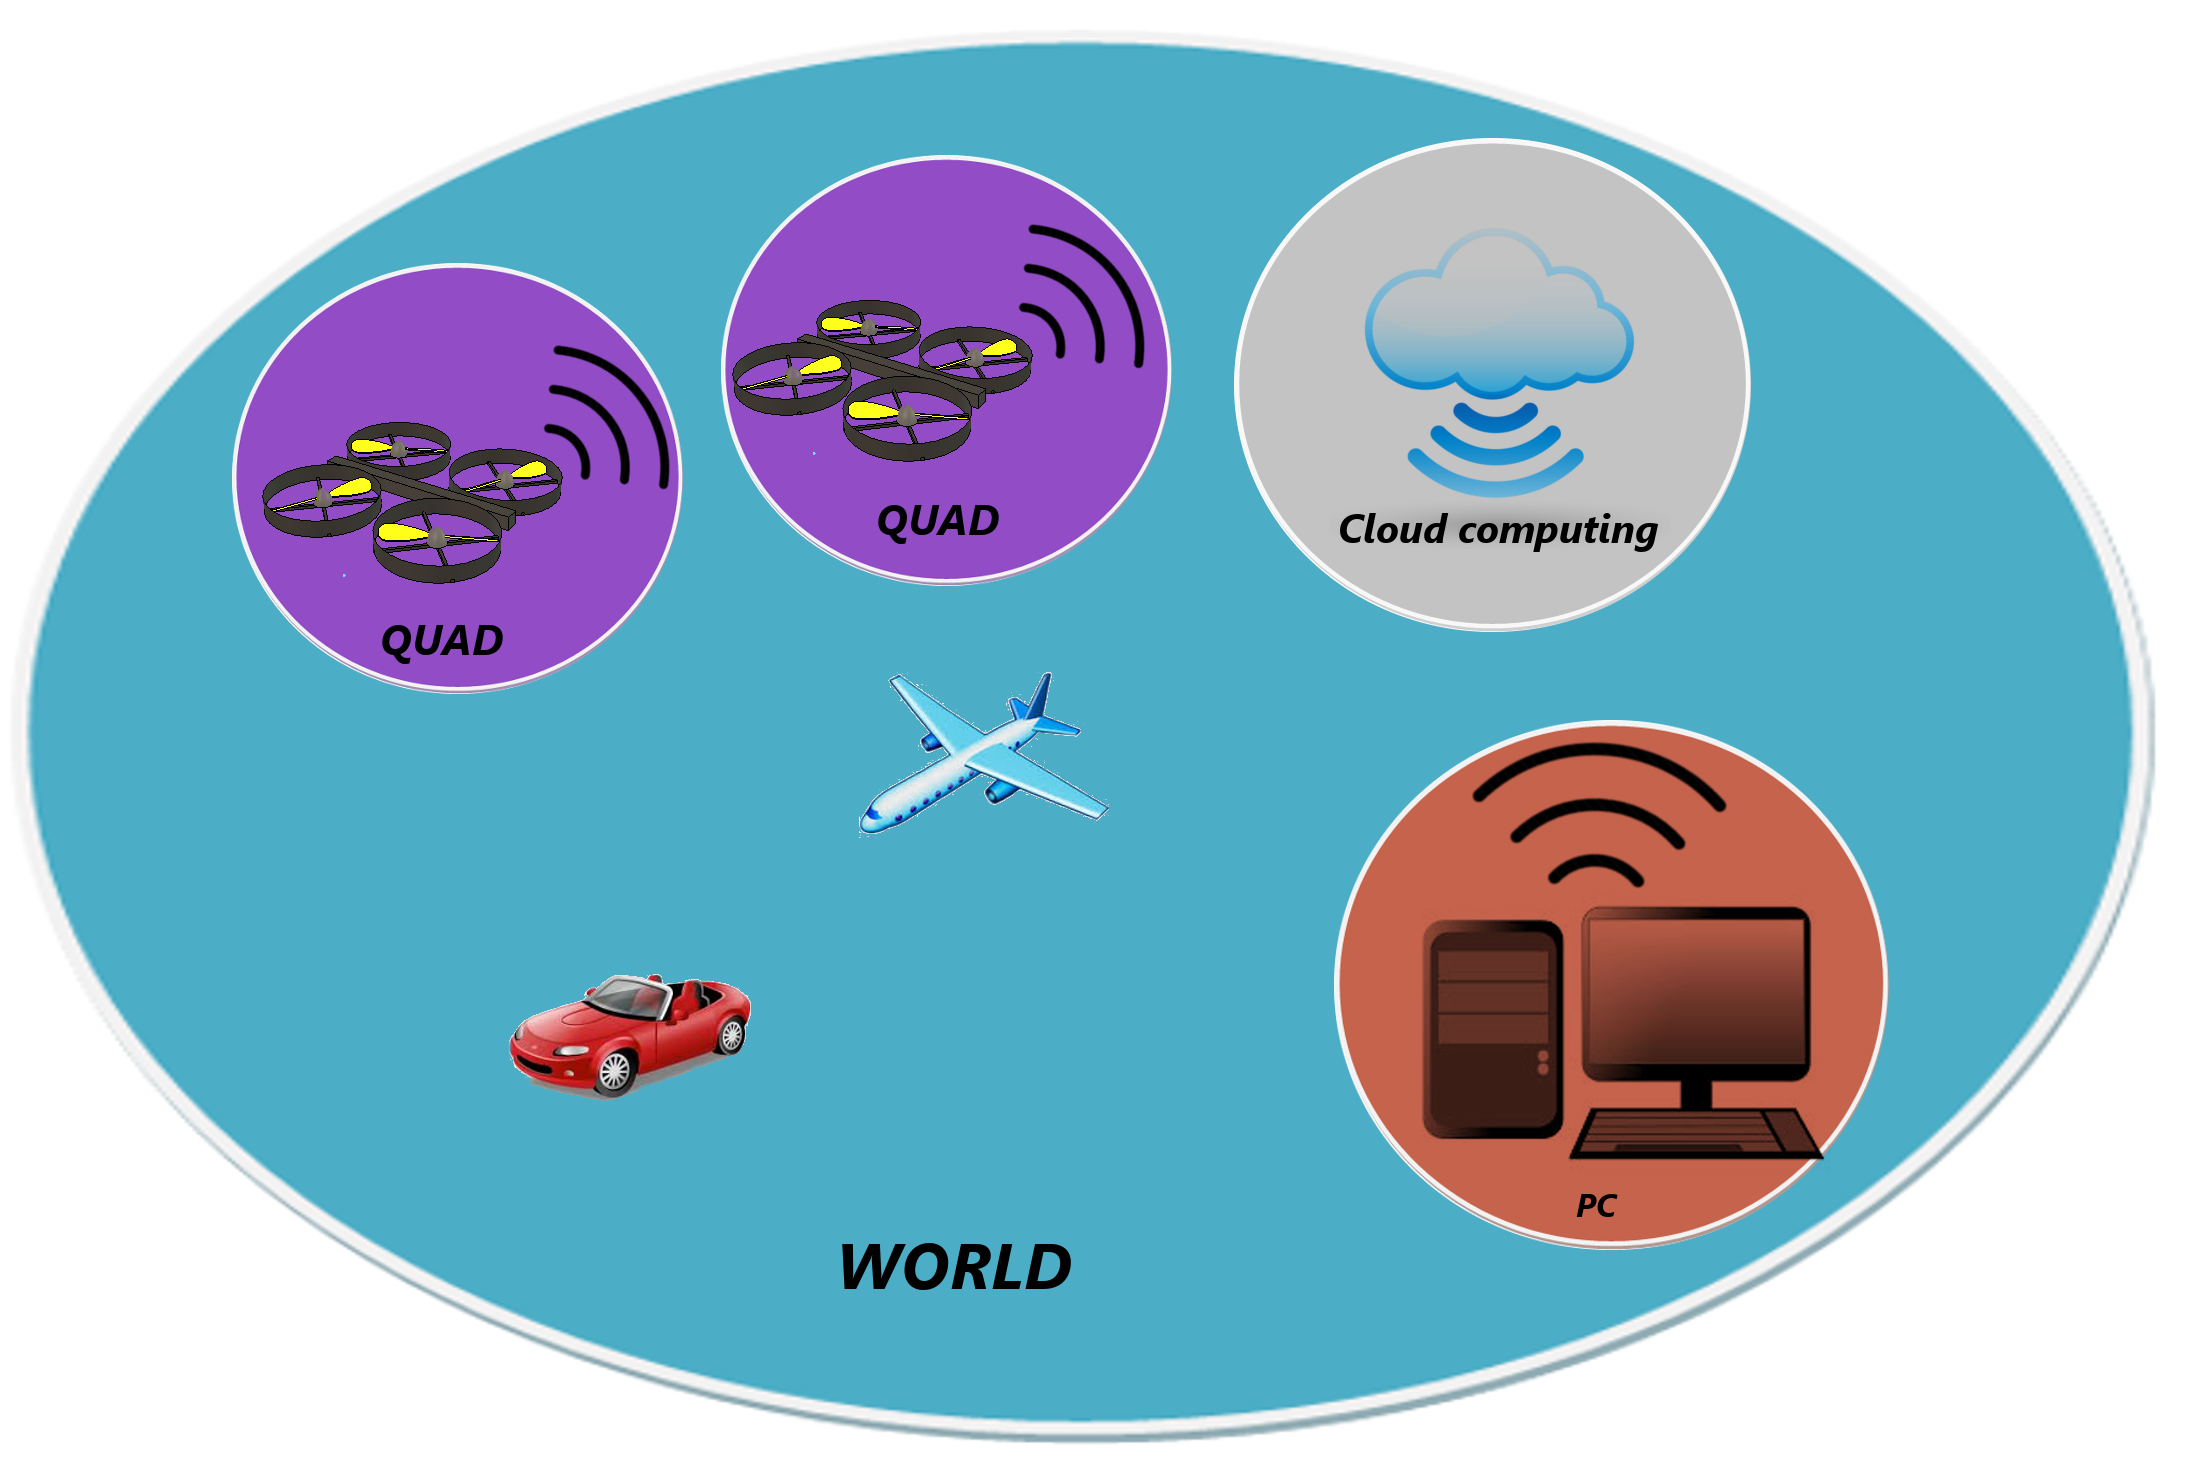
\includegraphics[width=0.50\textwidth,natwidth=220,natheight=1467]{../Images/c2/Architecture.png}
	\caption{System Architecture}
	\label{fig:System_Architecture}
\end{figure}


\begin{itemize}
  \item Set of quadrotors.
  \item Groundstation.
  \item Access Point (AP).
  \item Targets.
\end{itemize}

Every quadrotors has a camera and an embedded computer that runs the algorithm. Every frame, the algorithm segment the image and send to the ground station through the AP. The station process the received data and make an step on the tracking algorithm (EKF).

\newpage
\subsection{Quadrotors Software}

	\begin{figure}[hp]
		\begin{center}
			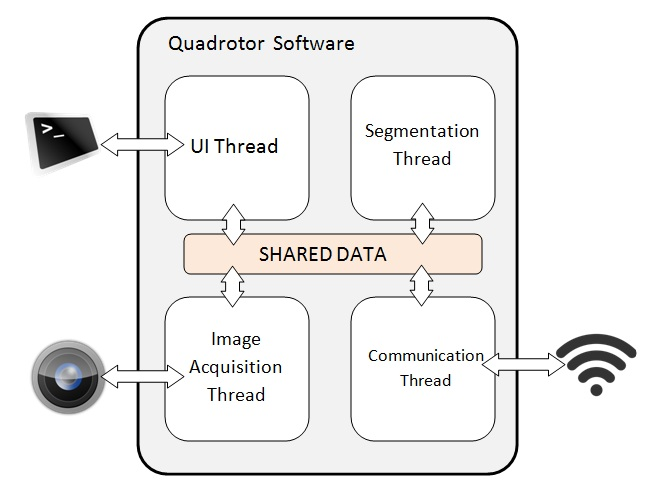
\includegraphics[width=0.7\linewidth]{../Images/c2/Quadsoftware}
		\end{center}
		\caption{Quadrotor's Software}
		\label{fig:Quadsoftware}
	\end{figure}

	Every Quadrotor will run an application \ref{fig:Quadsoftware} that is composed by a number of threads that allows it to parallelize the algorithm. This threads are:
	
	
	\begin{itemize}
		\label{itemize:quadappthreads}
		\item User interface thread.
		\item Image acquisition thread.
		\item Image segmentation thread.
		\item Communication thread.
	\end{itemize}
	
	
	
	The UI thread is a simple thread that display some options to get information about the process and also to stop it safely. The second thread handle the camera device and store it as soon as possible in order to allow the third thread to process images without delay. Eventually the communication thread send the information acquired on the previous process to the ground station through the TCP/IP connection.
	
\subsection{Ground Station Software}
	\begin{figure}[hp]
		\begin{center}
			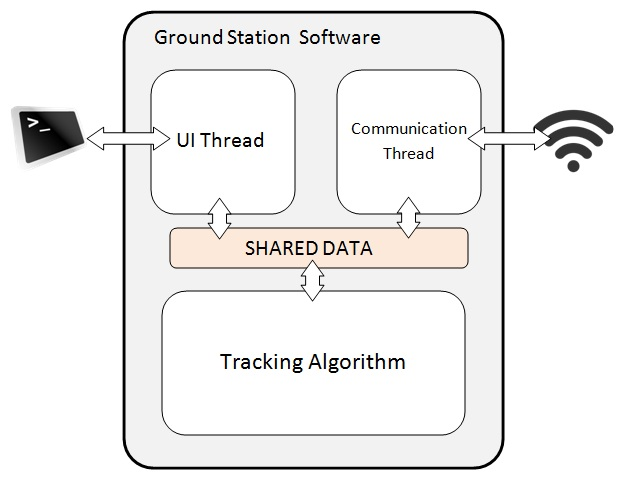
\includegraphics[width=0.7\linewidth]{../Images/c2/GroundStationsoftware}
		\end{center}
		\caption{Ground station's Software}
		\label{fig:GroundStation}
	\end{figure}

	On the ground station, as in quad's computer, there will be running an application with parallel threads that manage the information to run as fast as possible the tracking algorithm. This threads are:

	\begin{itemize}
		\item User interface thread.
		\item Communication thread.
		\item Tracking thread.
	\end{itemize}

	In this application, the UI thread has the same utility that the previous one (Request information about the process and stop the application safely). The communication thread manage all the input connections (Requests and input data messages). Then arrange the useful information to run the tracking algorithm.
	
\subsection{Conclusion}
The functionality of both, quads and station, can be easily modified by adding threads with access to the socket. For example, making the station to send the results of the EKF is as easier as send a message through the socket using the interface provided by BOViL \cite{BOViL}. 

In addition, the algorithm is designed with abstract interfaces from beginning, so any part of the architecture could be replaced by others with the same interface, for example:

\begin{itemize}
  \item Set of quadrotors $\Longrightarrow$ Set of quadrotors and ground vehicles.
  \item Ground Station $\Longrightarrow$ Multiple Ground Stations, cloud computation \cite{Cloud_computing} or even "inside quads" Station.
  \item Access Point (The router in this case) $\Longrightarrow$ GSM modules (For cloud computing or if operation is far away from the Station).
  \item Targets. Keep been any target.
\end{itemize}


% 666 TODO: terminar